\chapter{Capa de red}
Una vez explicada la parte hardware del proyecto, donde queda definido los diferentes sensores a usar, su colocación y conexión, y el controlador a usar, se va a explicar la parte del software, comprendida entre la capa de red y la capa de la nube.

\section{Configuración inicial de la red}

La red a utilizar para hacer la conexión tiene la siguiente característica:
\begin{itemize}
    \item \textbf{Dirección de red:} 192.168.1.0
    \item \textbf{Máscara de subred:} 255.255.255.0
    \item \textbf{Dirección de puerta de enlace:} 192.168.1.1
\end{itemize}

Dentro de esta red, se va a asignar una IP y un puerto a cada controlador. La dirección IP la va a utilizar para obtener conexión a la red, y el puerto se va a utilizar para crear una comunicación entre cada controlador por individual y el back-end.

El back-end simplemente necesita una dirección IP para conectarse a la red. Las direcciones y puertos utilizados mientras se desarrollaba el proyecto pueden ser visualizadas en la Tabla \ref{tab:port}.

\begin{table}[h]
    \centering
    \begin{tabular}{|l|c|c|}
        \rowcolor[gray]{.5}
        \hline
            \color{white}Localización del controlador&\color{white}Dirección IP&\color{white}Puerto  \\
        \hline
            Exterior del frigorífico&192.168.1.226&41234  \\
        \hline    
            Cajón de las verduras&192.168.1.227&41235  \\
        \hline    
            Cajón de las frutas&192.168.1.230&41238  \\
        \hline   
            Cajón del embutido&192.168.1.228&41236  \\
        \hline
            Cajón de los basares de la puerta&192.168.1.229&41237 \\
        \hline
            Back-end&192.168.1.225&4000 \\
        \hline
    \end{tabular}
    \caption{Presupuesto de la capa de neblina o niebla}
    \label{tab:port}
\end{table}

La forma de comunicación va a ser enviando paquetes UDP entre el back-end y los controladores usando las direcciones IP y los puertos. Estas IP y puertos son editables en el sistema, para adaptarse a la red en la que estos se conecten.

\section{Conexión entre el controlador y el back-end}

Cuando un sensor registra un valor nuevo y llega al controlador, éste debe de enviarlo al back-end. Entre el controlador y la base de datos hay un archivo JavaScript ejecutándose que es el encargado de recibir ese valor del controlador, y hacer acciones con éste, entre las cuales está el ser guardado en la base de datos.

Todos los controladores del sistema tienen una conexión unidireccional en sentido del controlador al back-end, que es usada para que los controladores envíen sus nuevos valores al back-end.

Adicionalmente, el controlador que tiene conectado el sensor RFID, tiene una conexión en sentido del back-end al controlador, siendo una conexión bidireccional. Esta se utiliza para recibir por ejemplo datos a escribir en la tarjeta, o acciones a realizar con una tarjeta escrita.

Existe un archivo JavaScript ejecutándose por cada controlador en el sistema. Cada uno recibe los valores del controlador y éste decide que acciones hacer en el back-end en función de éste. Este programa ejecutándose debe de tener una conexión entre el controlador y la base de datos para poder administrarla, esto se va a conseguir utilizando las IPs y puertos especificados en la Tabla \ref{tab:port}, además de diferentes librerías que se van a explicar a continuación que van a ayudar para establecer la conexión.

\subsection{WiFiUDP}
Esta librería nos permite enviar y recibir paquetes UDP con información desde el controlador. Inicialmente se guarda en una variable la IP y el puerto a la cual se va a enviar o recibir información, es decir, la IP del back-end y el puerto dependerá del controlador. Los métodos que proporcionaban esta librería son lo siguientes:

\begin{itemize}
    \item \textbf{beginPacket():} Se inicia la escritura de un paquete especificando la variable con la IP y el puerto donde se va a enviar.
    \item  \textbf{write():} Se especifica el contenido del paquete.
    \item  \textbf{endPacket():} Finaliza el paquete y lo envía.
    \item  \textbf{read():} Se utiliza para recibir paquetes UDP, especificando el buffer donde guardar la información que se va a recibir y el tamaño máximo de éste.
\end{itemize}

Con estos métodos, se puede enviar y recibir paquetes desde el controlador satisfactoriamente.

\subsection{Dgram}
Dgram\cite{thirtythird} es una librería muy parecida a WiFiUDP. Se utiliza para enviar y recibir paquetes UDP con información desde el back-end. Una vez que se tiene la librería implementada y un objeto de ésta creado, se puede asignar un puerto a ese servidor que va a hacer de intermediario entre el controlador y la base de datos. Se van a emplear los siguientes métodos:

\begin{itemize}
    \item \textbf{send():} Se va a usar para enviar paquetes, especificando la dirección IP y el puerto por donde se envía, además del contenido del paquete.
    \item \textbf{on():} Se va a usar para recibir paquetes, especificándole el primer parámetro con la palabra \textbf{‘message’}. En el segundo parámetro se obtendrá el paquete UDP, pudiendo leerlo y administrar la información recibida de éste. También se puede usar este método con el parámetro \textbf{‘listening’}, que se ejecutará cuando el servidor esté preparado para recibir paquetes, o usar \textbf{‘error’}, que se ejecutará cuando se produzca un error.
\end{itemize}

\subsection{Axios}
Se utiliza para enviar peticiones al back-end y realizar acciones con la base de datos. Esta librería fue explicada en la sección 1.3.5.5, por lo que simplemente se menciona para especificar su uso en esta capa de IdC. Se utiliza para guardar los datos obtenidos del controlador, o para obtener algún valor de la base de datos que sea necesario para el correcto funcionamiento de este archivo JavaScript.

\section{Código para comunicar el controlador y el back-end}
Como se ha mencionado anteriormente, se va a tener un archivo JavaScript que va a crear una comunicación entre el controlador y el back-end por cada controlador que tenga el sistema. Como se explicó en el apartado de controladores, se tiene cinco en este sistema, por lo que van a existir cinco servidores, cada uno con su puerto, que van a estar ejecutándose continuamente para procesar la información que les pueda llegar desde el controlador.

Estos cinco servidores tienen una parte en común. Se va a crear la instancia del servidor, además de tres llamadas al método \textbf{“on()”}. Una con el parámetro \textbf{‘error’} por si ocurre alguno, una con el parámetro \textbf{‘listening’} para que avise cuando el servidor esté listo, y otra con el parámetro \textbf{‘message’} para procesar el contenido de un paquete cuando llegue.

También existe un método llamado \textbf{checkControllerStatus()} que se ejecuta cada hora, y éste comprueba si ha llegado un paquete de confirmación por parte del controlador que envía automáticamente cada ocho horas. Si el método del servidor comprueba que en 24 horas no ha llegado ningún paquete de confirmación, se entiende que el controlador se ha quedado sin energía y genera un aviso que es enviado al usuario administrador del sistema a través del correo electrónico.

Adicionalmente, en el servidor que recibe los paquetes RFID, existe otra instancia más de \textbf{“Dgram”} para poder enviar paquetes, ya que esta conexión era bidireccional, y un método llamado \textbf{checkDietStatus()} que se ejecuta cada hora y comprueba si ha habido un cambio de parte del día. La mañana es entre las 00:00 y las 11:59, la tarde entre las 12:00 y las 19:59, la noche entre las 20:00 y las 23:59.

Si se produce un cambio en la parte del día, se envía un correo a todos los usuarios del sistema recordando la dieta estipulada para esa parte del día, y avisa si se ha quedado algún elemento sin consumir en la dieta de la parte del día anterior.

Lo que queda por explicar es que se hace cuando llega un paquete en el método \textbf{“on()”} con parámetro \textbf{‘message}’, que se hace con el contenido de ese paquete. La respuesta es que no se hará lo mismo con la información que llegue con un sensor magnético, que con un sensor de peso o un sensor RFID, por lo que las acciones a hacer con la información que llegue dependerán del sensor que haya producido esa información.


Independientemente del sensor, cuando llegue un paquete a cualquiera de los cinco servidores con una ‘A’ (ALIVE) como contenido, es un paquete que permite identificar que el controlador sigue con energía y no está ausente. Se registra la hora de llegada y luego en el método \textbf{checkController()} se valida que ha llegado este paquete.

\subsection{Sensor de peso}

Si el paquete proviene del sensor de peso, se registra el valor recibido en la base de datos y si el peso registrado es menor que el anterior, significa que se ha cogido un producto, y si hay un usuario identificado mediante RFID, se va a añadir a su actividad el producto sacado del frigorífico y se va a buscar si ese producto esta en su dieta. Si está, se aplica como producto consumido en su dieta. Además, si el peso registrado está por debajo de un umbral especificado por el administrador, se va a añadir a la lista de la compra el producto que esté en el peso. Si está por encima del umbral, se elimina de la lista.

\begin{figure}[h]
    \centering
    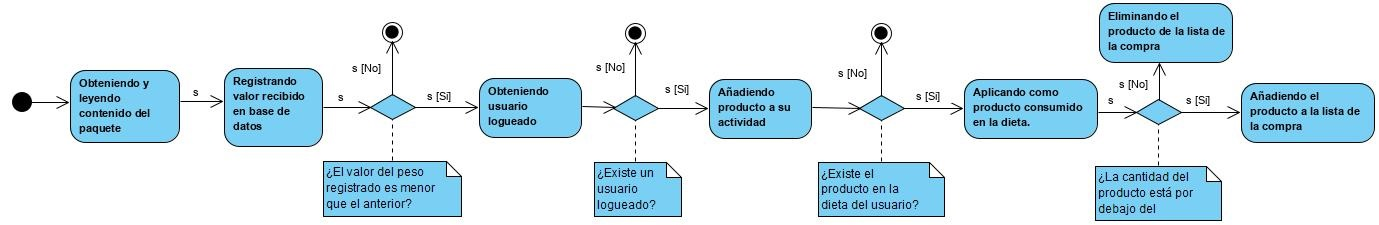
\includegraphics[width=\textwidth]{capitulos/capitulo7/diagramaPesoServer.jpg}
    \caption{Diagrama del proceso a seguir en un servidor cuando llega un paquete del sensor de peso.}
    \label{fig:diagramapesoserver}
\end{figure}

\subsection{Sensor de nivel}

Si el paquete proviene del sensor de nivel, si el valor es cero, significa que no hay agua, por lo que se registra el valor en la base de datos, y se añade a la lista de la compra (para rellenar el depósito). Si el valor es uno, se actualiza el valor en la base de datos y se elimina de la lista de la compra.

\begin{figure}[h]
    \centering
    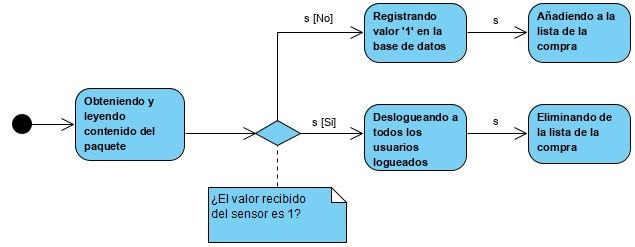
\includegraphics[width=.60\textwidth]{capitulos/capitulo7/diagramaNivelServer.jpg}
    \caption{Diagrama del proceso a seguir en un servidor cuando llega un paquete del sensor de nivel de agua.}
    \label{fig:diagramaaguaserver}
\end{figure}

\subsection{Receptor del sensor magnético}

Si el paquete proviene del sensor magnético de la puerta, se comprueba si el contenido es ‘1’. Si lo es, significa que la puerta está cerrada, y si el valor anterior era 0, significa que estaba abierta, por lo que se entiende que el usuario ha cerrado la puerta del frigorífico después de haberlo estado usándolo, por lo que se va a desloguear a cualquier usuario que estuviera logueado mediante RFID.

\begin{figure}[h]
    \centering
    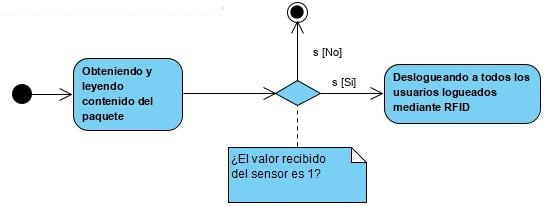
\includegraphics[width=.60\textwidth]{capitulos/capitulo7/diagramaMagneticoServer.jpg}
    \caption{Diagrama del proceso a seguir en un servidor cuando llega un paquete del sensor magnético.}
    \label{fig:diagramamagneticoserver}
\end{figure}

\subsection{Sensor RFID}
Si el paquete proviene del sensor RFID se pueden hacer varias cosas:
\begin{itemize}
    \item Si el paquete contiene una ‘I’ (INSERT), se debe de enviar un paquete al controlador con información para añadir a la tarjeta: 
    \begin{itemize}
        \item Si hay algún usuario preparado para registrar, se envía la información de éste para que el controlador haga el proceso de incorporar el contenido en la tarjeta, se elimina ese usuario de la cola de usuarios a añadir en tarjetas, y se modifica en la base de datos para especificar que el usuario está escrito en una tarjeta.
        \item Si no hay ningún usuario en la cola de usuarios a añadir en una tarjeta, se comprueba si hay algún producto para añadir. Si existe, se envía el ID del producto al controlador y se decrementa a una menos la cantidad a añadir de ese producto, o se elimina el producto directamente de la cola si era la última unidad para añadir.
        \item En caso de no haber ni productos ni usuarios para añadir, se envía un paquete con una ‘N’ (NOTHING) al controlador y se muestra por consola un mensaje.
    \end{itemize}
    \item Si el paquete recibido viene inicializado con un número, dependiendo del número se hará una acción u otra:
    \begin{itemize}
        \item Si el paquete viene iniciado con un 1, significa que se está introduciendo un producto en el frigorífico, por lo que se obtiene la ID del producto del paquete recibido y se aumenta una unidad más del producto con la ID que se ha recibido. Si el producto no existe, nos muestra un mensaje por consola.
        \item Si el paquete viene iniciado con un 2, significa que se está sacando un producto del frigorífico, por lo que se va a decrementar una unidad del producto. Al decrementar el número, en esa misma acción a nivel interno, se va a identificar si es necesario añadir ese producto a la lista de la compra si esta por debajo del umbral especificado por el administrador. Luego si hay un usuario identificado mediante RFID, se va a añadir a su actividad el producto sacado del frigorífico y se va a buscar si ese producto estaba en su dieta. Si estaba, se aplica como producto consumido.
        \item Si el paquete viene iniciado con un 3, significa que se está identificando un usuario con RFID:
        \begin{itemize}
            \item Si existe una petición de eliminado de ese usuario en esa tarjeta, se va a enviar un paquete al controlador especificando que se elimine el contenido de la tarjeta, y se va a actualizar el usuario para especificar que no tiene tarjeta.
            \item Si no existe una petición de eliminado, se envía un paquete al controlador especificando que no se elimine el contenido, y se actualizará el usuario a logueado. A partir de ese momento hasta que no se desloguee, se va a registrar todos los productos que se saquen del frigorífico en su usuario (el usuario se desloguea automáticamente al cerrar la puerta del frigorífico).
        \end{itemize}
    \end{itemize}
\end{itemize}

\begin{landscape}
    \vspace*{7em}
    \begin{figure}[h]
        \centering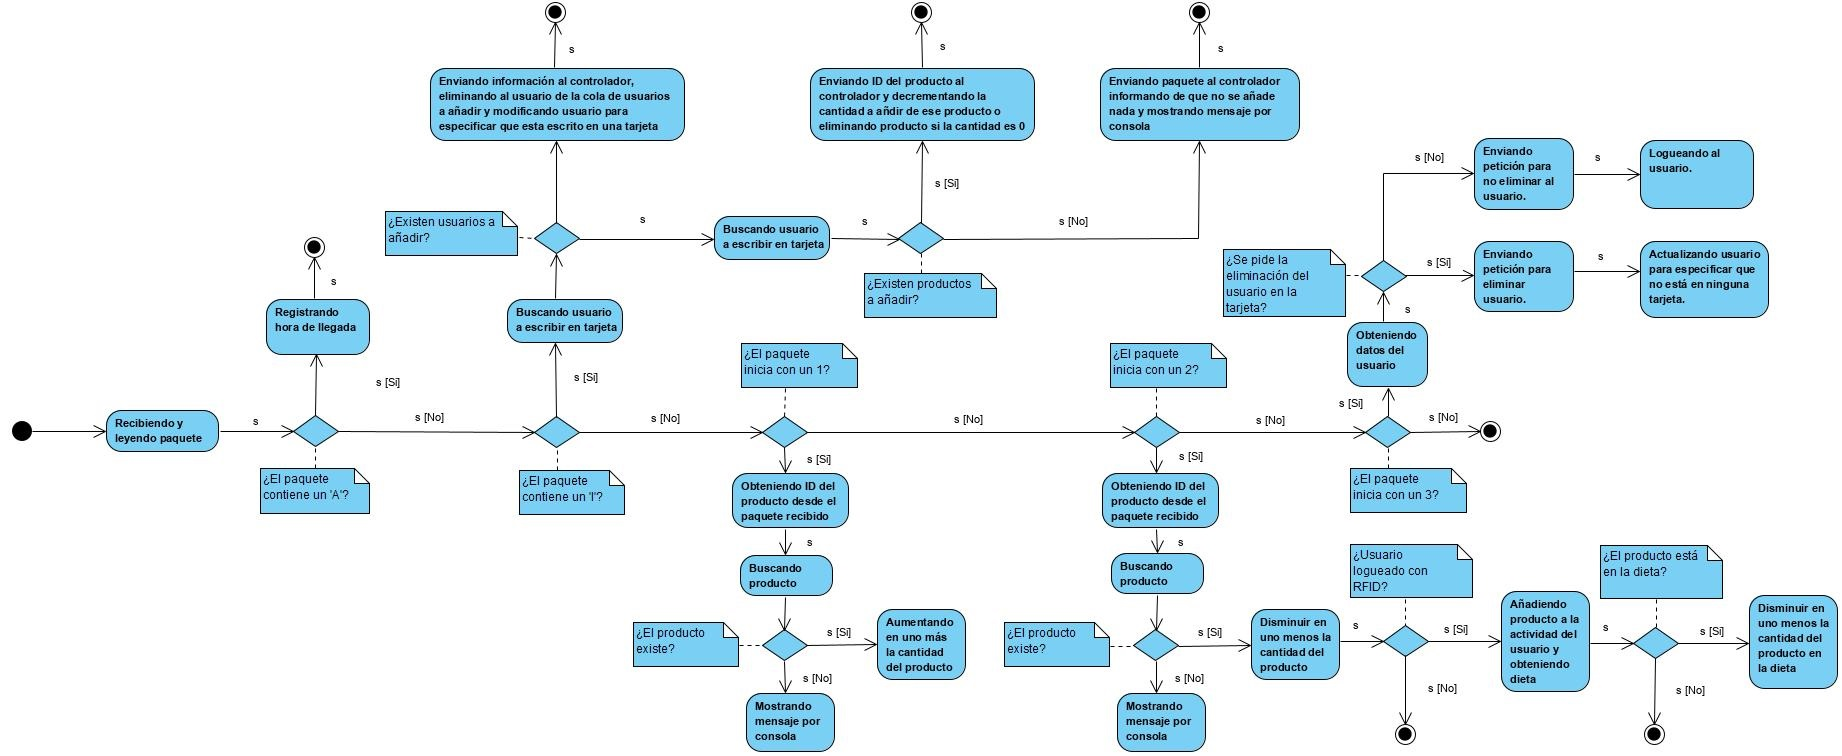
\includegraphics[width=\hsize]{capitulos/capitulo7/diagramaRFIDServer.jpg}
        \caption{Diagrama del proceso a seguir en un servidor cuando llega un paquete del sensor RFID.}
        \label{img_gantt}
    \end{figure}
\end{landscape}